% Figure 2: junction types in the canonical view.  Column width.  The numbers
% are the angles between the half-edge DIRECTIONS, one per pair.
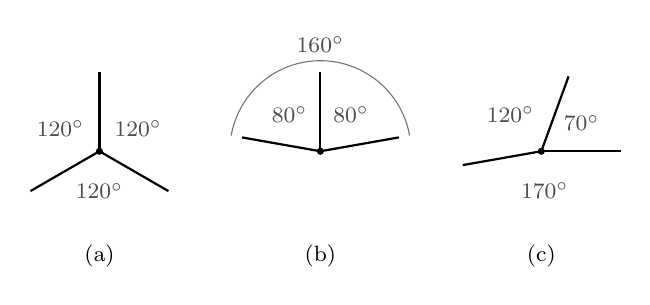
\begin{tikzpicture}[scale=0.92,font=\footnotesize]
  \tikzset{edge/.style={thick},ang/.style={black!70}}
  \begin{scope}[shift={(0,0)}]
    \foreach \a in {90,210,330} \draw[edge] (0,0) -- (\a:1.1);
    \fill (0,0) circle (1.4pt);
    \node[ang] at (150:0.62) {$120^\circ$};
    \node[ang] at (30:0.62)  {$120^\circ$};
    \node[ang] at (270:0.55) {$120^\circ$};
    \node at (0,-1.45) {(a)};
  \end{scope}
  \begin{scope}[shift={(3.05,0)}]
    \foreach \a in {10,90,170} \draw[edge] (0,0) -- (\a:1.1);
    \fill (0,0) circle (1.4pt);
    \node[ang] at (50:0.66)  {$80^\circ$};
    \node[ang] at (130:0.66) {$80^\circ$};
    \draw[black!55] (10:1.25) arc (10:170:1.25);
    \node[ang] at (90:1.47) {$160^\circ$};
    \node at (0,-1.45) {(b)};
  \end{scope}
  \begin{scope}[shift={(6.1,0)}]
    \foreach \a in {0,70,190} \draw[edge] (0,0) -- (\a:1.1);
    \fill (0,0) circle (1.4pt);
    \node[ang] at (35:0.68)  {$70^\circ$};
    \node[ang] at (130:0.66) {$120^\circ$};
    \node[ang] at (275:0.55) {$170^\circ$};
    \node at (0,-1.45) {(c)};
  \end{scope}
\end{tikzpicture}
